\section{Énergie transverse manquante}\label{chapter-HLO-section-MET}
\subsection{Définition}\label{chapter-HLO-section-MET-raw}
Des neutrinos peuvent être produits lors des collisions.
Or, ces particules se propagent sans laisser de signal dans le détecteur, elles sont donc invisibles.
Toutefois, lorsque de telles particules sont produites en association avec des particules détectées, leur présence peut être déduite du déséquilibre dans l'impulsion totale des particules de l'événement~\cite{CMS-PAS-JME-17-001}.
\par
La phénoménologie des collisions de protons est discutée chapitre~\refChLHCCMS.
Dans l'état initial,
la composante longitudinale de l'impulsion est inconnue
et
l'impulsion totale dans le plan transverse est nulle.
Par conservation, l'impulsion totale dans le plan transverse est nulle dans l'état final.
\par
Les neutrinos n'étant pas détectés, leurs impulsions transverses sont manquantes dans le bilan de l'état final.
L'observable définie afin de quantifier ce manque est
l'énergie transverse manquante (MET, \emph{Missing Transverse Energy}).
Bien que son nom mentionne une énergie, il s'agit bien d'une impulsion.
\par
La MET peut être déterminée à partir de l'algorithme de \PF\ (PF MET)
ou
par l'algorithme \PUPPI\ (\PUPPI\ MET).
Dans tous les cas, il s'agit de la MET brute qu'il faut corriger par la suite afin de conserver une description cohérente des événements lors de l'application des corrections des simulations comme exposé dans la section~\ref{chapter-HLO-section-MET-corr}.
\subsubsection{MET brute issue de l'algorithme \PF}
La somme des impulsions transverses des particules invisibles doit compenser celle des particules reconstruites, \ie
\begin{equation}
\sum_{\substack{\text{toutes les}\\\text{particules}}} \vpT = \vec{0}
\Leftrightarrow
\sum_{\substack{\text{particules}\\\text{invisibles}}} \vpT + \sum_{\substack{\text{particules}\\\text{reconstruites}}} \vpT = \vec{0}
\Leftrightarrow
\sum_{\substack{\text{particules}\\\text{invisibles}}} \vpT = -\sum_{\substack{\text{particules}\\\text{reconstruites}}} \vpT \mend
\end{equation}
\par La MET brute issue de l'algorithme \PF\ est ainsi définie comme
\begin{equation}
\vMET(\text{brute}, \text{\PF}) = -\sum_{i\in\set{\text{particules}}} \vpT^{(i)}
\mend[,]
\end{equation}
où les particules sont celles reconstruites par l'algorithme de \PF,
et représente l'impulsion transverse totale des particules invisibles.
Cette définition, simple, est toutefois sensible aux particules issues de l'empilement.
Afin de réduire l'effet de l'empilement, l'algorithme \PUPPI\ a été développé.
\subsubsection{MET brute issue de l'algorithme \PUPPI}
La MET peut également être estimée par l'algorithme \PUPPI\ (\emph{PileUp Per Particle Identification}) \cite{PUPPI}.
La \og \PUPPI MET \fg{} obtenue est moins sensible à l'empilement (\emph{pileup}) que la MET issue de l'algorithme de \PF\ (PF MET).
L'algorithme \PUPPI\ exploite en effet des informations sur:
\begin{itemize}
\item l'environnement de chaque particule identifiée par l'algorithme de \PF\;
\item les propriétés de l'empilement dans l'événement;
\item les données issues du trajectographe;
\end{itemize}
afin d'associer un poids $w_i$ à chaque particule $i$, lié à la probabilité que celle-ci proviennent de l'empilement au lieu du vertex primaire principal.
Ce poids varie entre
\num{0} pour des particules issues de l'empilement
et
\num{1} pour des particules provenant du vertex primaire principal.
Plus de détails dans la détermination de $w_i$ sont disponibles dans les références~\cite{CMS-PAS-JME-17-001,PUPPI}.
\par La MET brute issue de l'algorithme \PUPPI\ est définie comme
\begin{equation}
\vMET(\text{brute}, \text{\PUPPI}) = -\sum_{i\in\set{\text{particules}}} w_i\,\vpT^{(i)}
\mend
\end{equation}
\subsection{Corrections de l'énergie transverse manquante}\label{chapter-HLO-section-MET-corr}
\paragraph{Énergie des jets}
La correction en énergie des jets, abordée dans les sections suivantes, doit être propagée à \MET.
Cette propagation est faite selon
\begin{equation}
\vMET(\text{corr.}) = \vMET(\text{brute}) - \sum_\text{jets} \left( \vpT^\text{corr.} - \vpT^\text{non corr.} \right)
\end{equation}
où
\og non corr. \fg{} correspond aux observables avant correction
et
\og corr. \fg{} après correction.
\paragraph{Recul de \MET\ (\emph{MET recoil corrections})}
La modélisation de \MET\ dans certains jeux de données simulées (production du boson de Higgs, Drell-Yan (boson \Zboson) et \Wjets) ne correspond pas aux observations dans les données réelles.
Des corrections sur $\vec{U}$, défini comme la différence entre \MET\ et la somme des impulsions des neutrinos provenant de la désintégration du boson de Higgs, \Zboson\ ou \Wboson, \ie
\begin{equation}
\vec{U} = \vMET - \sum_{\nu_i \leftarrow \higgs,\Zboson,\Wboson} \vpT^{(\nu_i)}
\mend[,]
\end{equation}
sont appliquées pour corriger cet effet.
\par
Les composantes colinéaire $U_1$ et orthogonale $U_2$ du vecteur $\vec{U}$ à l'impulsion du boson sont déterminées dans des événements $\Zboson\to\mu\mu$ dans lesquels il n'y a pas de neutrino provenant de la désintégration du \Zboson, ce qui permet de mesurer précisément son impulsion.
L'écart à zéro de $U_1$ ainsi que la résolution sur $U_1$ et $U_2$ sont ainsi déterminés dans les données réelles et simulées.
Les données simulées sont alors corrigées afin de faire correspondre en moyenne ces valeurs à celles observées dans les données réelles.
Ces moyennes sont déterminées sur des intervalles d'impulsion du \Zboson\ ($[\num{0}, \num{10}[$, $[\num{10}, \num{20}[$, $[\num{20}, \num{30}[$, $[\num{30}, \num{50}[$ et $>\SI{50}{\GeV}$) et du nombre de jets ($\Njets\in\set{0, 1, \geq2}$).
\par
L'effet de cette correction sur une sélections d'événements $\Zboson\to\mu\mu$ en 2017 est présenté sur la figure~\ref{fig-MET_recoil_Alexei}.
Les distributions observées (données réelles) et modélisées (données simulées) de \MET\ y sont tracées.
L'accord entre observation et modélisation, dont le rapport (obs/exp) est également donné, est sensiblement amélioré par cette correction.
\begin{figure}[h]
\centering

\subcaptionbox{Distribution de \MET\ sans correction.}[.45\textwidth]
{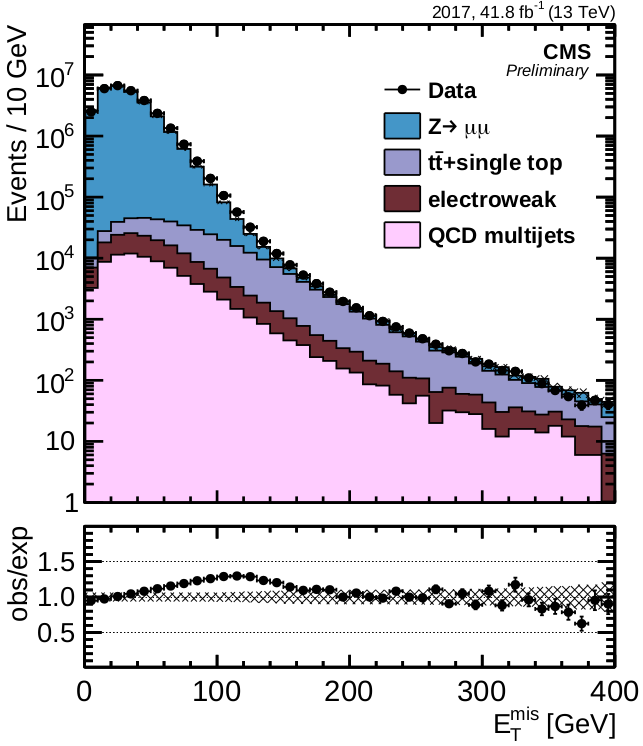
\includegraphics[width=.45\textwidth]{/home/torterotot/Documents/PhD-Thesis/plots_and_images/from_MET_recoil_Alexei/withoutrecoil.png}}
\hfill
\subcaptionbox{Distribution de \MET\ avec correction.}[.45\textwidth]
{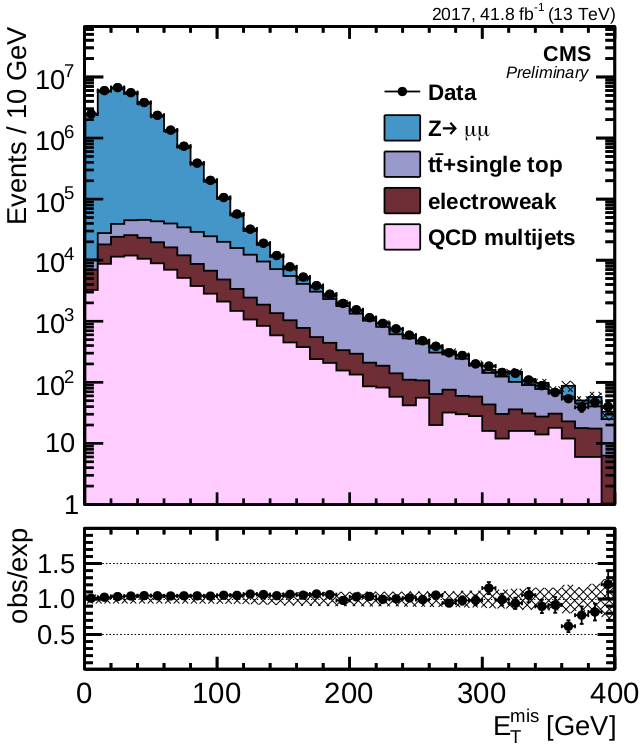
\includegraphics[width=.45\textwidth]{/home/torterotot/Documents/PhD-Thesis/plots_and_images/from_MET_recoil_Alexei/withrecoil.png}}

\caption[Effet de la correction de recul de \MET.]{Effet de la correction de recul de \MET\ sur une sélection d'événements $\Zboson\to\mu\mu$ en 2017~\cite{MET_recoil_Alexei}.}
\label{fig-MET_recoil_Alexei}
\end{figure}